\documentclass[letterpaper]{article} % DO NOT CHANGE THIS
\usepackage[submission]{aaai2027} % DO NOT CHANGE THIS
% The serif, sans-serif, and monospaced fonts are loaded automatically by
% aaai2027.sty (newtxtext, helvet, courier). DO NOT add \usepackage{times},
% \usepackage{helvet}, \usepackage{courier}, or any other font package.
\usepackage[hyphens]{url} % DO NOT CHANGE THIS
\usepackage{graphicx} % DO NOT CHANGE THIS
\urlstyle{rm} % DO NOT CHANGE THIS
\def\UrlFont{\rm} % DO NOT CHANGE THIS
\usepackage{natbib} % DO NOT CHANGE THIS AND DO NOT ADD ANY OPTIONS TO IT
\usepackage{caption} % DO NOT CHANGE THIS AND DO NOT ADD ANY OPTIONS TO IT
\frenchspacing % DO NOT CHANGE THIS

% Math / theorems / tables (compatible with aaai2027.sty)
\usepackage{amsmath,amssymb,amsthm}
\theoremstyle{plain}
\newtheorem{theorem}{Theorem}
\newtheorem{proposition}{Proposition}
\usepackage{booktabs}

\newcommand{\wcrit}{w_{\mathrm{crit}}}
\newcommand{\PT}{\mathrm{PT}}

\setcounter{secnumdepth}{0}

\title{Measuring Coordination-Collapse Boundaries in Reward-Mixed Cooperative MARL}

\author{
  Anonymous Submission
}
\affiliations{}

\begin{document}

\maketitle

% =======================================================================
\begin{abstract}
Cooperative multi-agent reinforcement learning can settle into low-cooperation lazy-agent behavior when
agents' local incentives dominate the team objective. We study not only whether reward centralization
mitigates this failure, but where a trained population crosses into a pre-specified collapse region.
We sweep the local-to-team reward mixture $w$, estimate $P(\mathrm{collapse}\mid w)$, and report the
midpoint $\wcrit$ with bootstrap confidence intervals; on our primary supply-chain testbed,
$\wcrit=0.666$ $[0.635,0.694]$. Using this boundary instrument, we evaluate a loss-averse reward
transform that weights losses more heavily than equal-sized gains. On the primary testbed, we separate
this effect from value-function curvature, which moves the boundary in the opposite direction. Across
four environment--algorithm combinations, the loss-aversion direction persists, while longer training
horizons move the boundary leftward. The thresholds are specific to the environment, learner, training
budget, reward units, and collapse label, but the protocol provides a reusable instrument for locating
coordination failure and measuring how reward transformations and learning conditions move its boundary.
\end{abstract}

% =======================================================================
\section{Introduction}
\label{sec:intro}

A team of learning agents can fail even when the task has a good cooperative solution: instead of
learning complementary behavior, agents can settle into locally safe, low-cooperation behaviour.
We call this \emph{coordination collapse};
in the MARL literature its endpoint is the \emph{lazy-agent}
policy~\citep{liu2023lazy,peng2023curo}, and the underlying private-versus-collective conflict is
the one studied in sequential social dilemmas~\citep{leibo2017multi}. We study this failure through
a \emph{reward-centralization} dial: within each reward-mixing sweep, agent $i$ is trained on the
blended scalar $x_i(w)=(1-w)\,r_i^{\mathrm{local}}+w\,r^{\mathrm{global}}$, $w\in[0,1]$, so at
$w{=}0$ the learner sees only its own local reward and at $w{=}1$ only the team reward. Turn $w$
down and an agent's private performance drowns out its contribution; cooperating earns no
learnable signal and the lazy policy wins. That decentralized reward shaping cannot match
centralized training is broadly accepted~\citep{dmarl2025}, and lazy-agent and credit-assignment
work~\citep{liu2023lazy,peng2023curo,sunehag2018vdn,rashid2018qmix,foerster2018counterfactual}
mitigates the pathology; what none of it supplies is the \emph{location}. The closest phase-diagram
studies place their critical points on \emph{environmental}~\citep{yamaguchi2025} or
opinion-dynamics~\citep{capannoli2026phase} axes rather than reward structure, and none estimates a
confidence-intervalled crossing in reward-centralization space for gradient-trained cooperative
policies. Our central question is therefore twofold: does coordination collapse admit a
\emph{measurable} critical centralization threshold $\wcrit$, and do prospect-theoretic reward
transforms systematically shift it? The first is a measurement problem (the paper's primary
contribution); the second is a question the instrument then makes answerable.

Pinning down this number matters because reward design is not neutral. $\wcrit$ is not universal: it
is a measured property of an environment, learner, horizon, and collapse label that tells a designer
where their own system crosses into collapse. We estimate it in four environment-algorithm
combinations (a six-node inventory network under PPO and MAPPO, and Cooperative Navigation (MPE) and
Level-Based Foraging (LBF) under MAPPO). Because the boundary is finite-horizon, we also re-measure it
across horizons on the primary supply-chain testbed and the two transfer environments. The inventory network is a branching directed-flow graph, which later lets us ask
\emph{which} node's reward design sets the boundary. We use prospect theory only as a controlled
reward-transform family, not a psychological claim: precisely, a pointwise loss-asymmetric transform
of the immediate blended reward, omitting the probability-weighting channel of full prospect
theory. After blending, the scalar is transformed with value-function curvature and loss aversion (a
loss looming larger than an equal gain~\citep{kahneman1979,tversky1992}), while the learner,
architecture, optimizer, and evaluation label are unchanged. The experimental question is then clean: does changing the scalar training
signal move the collapse boundary?

We build the instrument before using it. Three design choices make a reading trustworthy: the collapse
label is a behavioral rule scored on evaluation and pre-registered on the primary supply-chain testbed
(label, analysis code, and probes committed before execution); matched policies differ only in the
scalar training signal, since the transform is applied after blending, outside the optimizer; and every
$\wcrit$ carries a bootstrap confidence interval. We use ``boundary'' in this operational sense: a
finite-training, threshold-defined behavioral crossing in learning dynamics, not a claim of phase-like
criticality.

The contributions are: (i)~a confidence-intervalled protocol for locating collapse boundaries in
reward-mixed cooperative MARL; (ii)~a controlled reward-transform decomposition showing that
value-function curvature and loss aversion can move the boundary in opposite directions, while the
loss-aversion direction replicates across four environment--algorithm combinations and the
finite-horizon slide recurs on the primary supply-chain testbed and both transfer environments; and
(iii)~a scoped heterogeneity result showing that, under parameter sharing on the
supply chain, one loss-averse node can nearly set the team boundary, while a separate-actor control
rules out a general topology-based ordering. Magnitudes and secondary structure are substrate-specific
unless separately replicated. The contribution is not the logistic midpoint itself, but a comparative
protocol for measuring how training choices and reward transformations move a system-level failure
boundary, with uncertainty.

% =======================================================================
\section{Related Work}
\label{sec:related}

Cooperative MARL, studied since independent $Q$-learning on shared
tasks~\citep{tan1993multi,busoniu2008comprehensive}, inherits the lazy-agent and
relative-overgeneralization failures in which agents abandon cooperation for a degenerate
policy~\citep{liu2023lazy,peng2023curo,tampuu2017multiagent}. The standard remedy is centralized
credit assignment under CTDE, a centralized critic or factorized value
function~\citep{lowe2017multi,yu2022surprising,sunehag2018vdn,rashid2018qmix,foerster2018counterfactual,son2019qtran};
related work ties the failure to
decentralized exploration~\citep{weng2026} or shows decentralized shaping cannot match centralized
baselines~\citep{dmarl2025}. This establishes \emph{that} centralization helps and \emph{how} to
implement it; none locates the threshold $\wcrit$ or gives it a confidence interval, the gap we
close, using $w$ as the dial rather than a fixed factorization. Combined individual-and-team reward
design has direct precedent: DE-MADDPG separates a per-agent and a team critic for exactly such
mixtures~\citep{demaddpg2020}, and packet-routing work has used RL routing as a testbed and later
studied the lazy-versus-selfish trade-off with mixed and adaptive local/global
signals~\citep{packetrouting,mao2020reward}; but these set or adapt
the mixture as a design choice rather than \emph{locating} $\wcrit$ or giving it a confidence
interval.

Treating collective learning as a dynamical system with critical points has
precedent: \citet{yamaguchi2025} builds a phase diagram for independent Q-learning over
\emph{environmental} axes, and \citet{capannoli2026phase} prove a metastable boundary in opinion
dynamics under a fixed update rule. Mean-field and dynamical-systems analyses derive deterministic or
distributional limits for multi-agent learning~\citep{hu2019meanfield,barfuss2019deterministic,hussain2025convergence}.
We borrow the phase-diagram measurement style but differ in object: ours is a \emph{reward-structure}
threshold with confidence intervals, and we use the mean-field machinery only for a sign-level account
(Supplement).

The heterogeneous-node result also has adjacent precedent in threshold and cascade models. Aggregate
outcomes can depend on the distribution of actors' thresholds rather than their average
preferences~\citep{granovetter1978threshold}, while small initial shocks can produce global cascades in
susceptible networks~\citep{watts2002global}. We use this literature only as conceptual precedent, not
as evidence of a cascade mechanism in our setting. Our contribution is to measure how assigning a
loss-averse reward transform to a single node shifts a finite-training coordination-collapse boundary in
gradient-trained cooperative MARL; moreover, a separate-actor control rules out a general
topology-based ordering.

Human preference structure has entered collective learning only narrowly.
\citet{hughes2018inequity} show inequity aversion improves cooperation within the cooperative-AI
agenda~\citep{dafoe2020open,hammond2025multiagent,barfuss2020caring}, and loss aversion is now a
training objective at scale: KTO aligns language models with a Kahneman--Tversky value function
carrying an explicit loss-aversion coefficient~\citep{ethayarajh2024kto}. Risk-sensitive RL optimizes
tail outcomes~\citep{qiu2021rmix,xie2023riskq,prashanth2014cvar,tamar2015optimizing} (distinct from
loss aversion's reference-point asymmetry), and prospect theory has entered single-agent RL with known
calibration concerns~\citep{prashanth2016cumulative,rabin2000risk,tversky1992}. In multi-agent settings,
\citet{mengesha2025} find loss aversion \emph{non-monotone} in an evolutionary quantal-response model,
and \citet{lalmohammed2025} bring CPT into cooperative MARL but fold it into the actor--critic update,
varying value and probability-weighting components jointly with the optimizer. We differ at the level of \emph{apparatus}: rather than proposing
another behavioral model, we build a measured boundary and use it as a common instrument; the
prospect-theoretic reward-transform study is its first application, not the instrument's whole
contribution.

% =======================================================================
\section{Preliminaries and Method}
\label{sec:method}

We study \emph{reward-mixed} cooperative MARL, in which each learner's scalar reward is the blend
$x_i(w)=(1-w)\,r_i^{\mathrm{local}}+w\,r^{\mathrm{global}}$, $w\in[0,1]$; our primary supply-chain
learner is parameter-shared PPO (a shared actor--critic with per-agent observations and
decentralized execution; ``IPPO'' in the shared-parameter sense) and the transfer settings use a
centralized critic. Here $w$ is not an
optimizer hyperparameter but a structural property of the reward design. We do not rescale
$r_i^{\mathrm{local}}$ or $r^{\mathrm{global}}$ separately at each $w$; both stay in the
environment's native units, so a given $w$ means the same mixture in every condition rather than
hiding a per-condition normalization. Unless stated otherwise, each experiment varies one factor at
a time, holding the learner, environment, horizon, transform parameters, and label fixed.

The boundary estimate follows four steps: fix the environment, learner, horizon, and collapse
label; train matched policies across a grid of $w$; label each run from pre-specified
\emph{evaluation} behavior, not training reward; and fit a monotone binary model
$P(\mathrm{collapse}\mid w)$, reporting the midpoint $\wcrit$ with bootstrap confidence intervals.

The reward transform is prospect-theoretic in value-function form: with zero as the gain/loss
reference, $v(x)=x^\alpha$ for $x\ge0$ and $-\lambda(-x)^\beta$ for $x<0$. The exponents
$\alpha,\beta\in(0,1]$ control \emph{curvature} (values below one make the transform sublinear, compressing
larger magnitudes); the separate multiplier $\lambda>1$ scales the entire loss branch, so a loss counts $\lambda$
times an equal gain (\emph{loss aversion}), and $\alpha{=}\beta{=}1,\lambda{=}1$ leaves $v(x)=x$.
Because curvature is present in every loss-aversion condition, we run a curvature-only baseline so its
effect is not silently folded into the $\lambda$ shift. We omit the probability-weighting channel of
full CPT, so only the scalar value transform varies between matched runs. Applied after blending,
\begin{equation}
 r_i^{\PT}=v\!\left((1-w)\,r_i^{\mathrm{local}}+w\,r^{\mathrm{global}}\right),
 \label{eq:reward}
\end{equation}
this keeps the optimizer and architecture bit-identical across matched conditions, the difference
from \citet{lalmohammed2025}, who embed CPT \emph{inside} the actor--critic update, varying transform,
probability weighting, and optimizer together. A measured shift is thus attributed to the transform
channel, while recognizing that reward scale, variance, and advantage shape are part of that channel.

A \emph{collapse label} is a pre-specified binary evaluation rule marking runs whose behavior lies
inside a low-cooperation region, scored on held-out evaluation episodes rather than training reward.
In the supply chain, collapse is $\mathbf{1}[\bar S<10\wedge\bar\pi\le-127.1]$, with $\bar S$ the
mean base-stock and $\bar\pi$ the mean profit over deterministic evaluation; this corresponds to
low/no ordering with poor profit. Collapsed runs pile up at the lazy-policy deterministic
profit floor ($\approx-128$), so the profit clause is effectively a redundancy check on
$\bar S<10$ rather than a tuned cutoff. In MPE (Cooperative Navigation), collapse is landmark
occupancy below $\theta=0.144$, i.e.\ agents cluster rather than cover landmarks; in LBF
(Level-Based Foraging), collapse is mean team return below $\theta=0.626$ (the calibrated
collapsed-versus-coordinated midpoint), i.e.\ agents fail to cooperatively load food. The supply-chain
label and analysis code were frozen before execution; threshold robustness over estimable $\pm20\%$
variants changes $\wcrit$ by at most $0.015$ (Supplement).

For each condition we fit $P(\mathrm{collapse}\mid w)=\sigma(b_0+b_1 w)$ and report
$\wcrit=-b_0/b_1$, the $w$ at which fitted collapse probability is $0.5$, with percentile-bootstrap
CIs over runs~\citep{efron1993bootstrap} ($2{,}000$ resamples). Where collapse is near-perfectly
separated across adjacent $w$ (steep high-$\lambda$ cells) the ordinary slope diverges, so those cells
use Firth's bias-reduced logistic regression~\citep{firth1993}, whose $\wcrit$ agrees with the
bootstrap to within $0.019$. The location is not an artifact of the logistic link: a probit link and
isotonic (nonparametric monotone) regression reproduce $\wcrit$ to within $0.02$ at every $\lambda$ on
all three substrates, and the $\lambda{=}1{\to}7$ shift is unchanged under all three (Supplement). The
transition width is the fitted 10--90 width $\Delta w=(\mathrm{logit}(0.9)-\mathrm{logit}(0.1))/|b_1|$.
The decomposition compares, at identical environment and optimizer, a \textbf{linear baseline}
($\alpha{=}\beta{=}1,\lambda{=}1$), a \textbf{curvature baseline} ($\alpha{=}\beta{=}0.88,\lambda{=}1$),
and \textbf{loss-aversion conditions} ($\alpha{=}\beta{=}0.88,\lambda>1$). The primary substrate is
\texttt{NetworkManagement-v1}~\citep{hubbs2020orgym}, a six-node multi-echelon inventory
network~\citep{oroojlooyjadid2022,gijsbrechts2022,marlim2023}, chosen because it exposes a
directed-flow failure and supports the minority-topology analysis; transfer environments are MPE
Cooperative Navigation~\citep{lowe2017multi} and Level-Based Foraging~\citep{christianos2020shared}.
Supply-chain agents run parameter-shared PPO~\citep{schulman2017ppo} via
Stable-Baselines3~\citep{raffin2021sb3}; MPE, LBF, and the cross-algorithm control for supply chain use MAPPO (PPO with
a centralized critic~\citep{yu2022surprising}) on the same stack, all wrapped with
PettingZoo/SuperSuit~\citep{terry2021pettingzoo,terry2020supersuit}. Headline $\lambda$ sweeps use
$20$ seeds per $(w,\lambda)$ cell; the full run inventory is in the Supplement. Primary results are
supply-chain/PPO; the supply-chain/MAPPO, MPE/MAPPO, and LBF/MAPPO settings are transfer tests of
which claims generalize (Table~\ref{tab:generalization}).

% =======================================================================
\section{The Boundary and Its Reward-Transform Shift}
\label{sec:results}

\paragraph{A well-defined boundary exists at fixed training budget.}
At 300k steps on the supply-chain PPO substrate, collapse has a clear, tightly-estimated boundary in
reward-centralization space (Figure~\ref{fig:boundary}a): the fitted midpoint is $\wcrit=0.666$
$[0.635,0.694]$, and three
independent estimators, logistic, probit, and isotonic (nonparametric monotone) regression, agree to
within $0.02$ (Method), a stronger check than any single link-function fit. The transition is
monotone with a $10$--$90$ width of $\Delta w=0.199$ (about a fifth of the mixture axis); a Firth
logistic-slope test also rejects the (much weaker) null of no relationship between $w$ and collapse
at all ($p=3.2\times10^{-7}$): a resolved, non-flat crossing rather than
phase-like sharpness. We use 300k as the primary horizon; horizon dependence is measured below.

\paragraph{``Collapse'' is an operational threshold crossing, not a confirmed attractor.}
A fitted midpoint exists whenever the binary label varies with $w$, so we tested the underlying
continuous behavior for a distinct dynamical regime: bootstrap 95\% CIs on Sarle's bimodality
coefficient~\citep{sarle1983cluster} and Hartigan's dip test~\citep{hartigan1985dip} against a
unimodal null, across both substrates and all $w$ (Supplement). On the supply chain Sarle's coefficient
rises near the crossing (0.59 at $w{=}0.65$ and 0.57 at $w{=}0.75$, both above the 0.555 rule-of-thumb)
but its CI straddles the threshold
everywhere, and the dip test never rejects unimodality ($p\ge0.30$). LBF's raw team return shows
nominally significant dip statistics at high $w$ ($p<0.05$), but this traces to a ceiling effect (runs
saturating at the metric's upper bound), not a second basin: excluding ceiling-clipped runs removes
the significance ($p\ge0.11$). Neither substrate clears a formal multimodality test at our sample
sizes, so we drop the attractor language and use \emph{threshold-defined behavioral crossing}
throughout.

\paragraph{The boundary is finite-horizon.}
The boundary slides left with the training horizon: across four matched risk-neutral horizons
$\wcrit=0.822,0.666,0.622,0.573$ at $150/300/450/900\mathrm{k}$ steps, log-linear in $T$
($\wcrit=2.44-0.138\ln T$, RMSE $0.027$; all four CIs of width ${\le}0.073$; Figure~\ref{fig:boundary}b).
Longer training rescues some runs that collapse at shorter horizons; at any fixed budget $\wcrit$ is
well-defined, so horizon dependence does not make it arbitrary. The log-linear fit is local to the
tested range ($150$k--$900$k, a single
order of magnitude); we use it to summarize the measured slide, not to extrapolate an asymptotic
boundary. Mechanistic escape interpretations are treated only as supplementary, non-load-bearing
explanations.

\paragraph{The horizon slide is not a supply-chain artifact.}
Under centralized-critic MAPPO the same slide recurs in both transfer environments: on MPE $\wcrit$
falls $0.82\to0.68$ over $2\mathrm{M}\to8\mathrm{M}$ steps, and on LBF $0.33\to0.20$ over
$1\mathrm{M}\to4\mathrm{M}$, both with non-overlapping endpoints. A basin control rules out the
confound that runs collapse because they start closer to the lazy basin: within each $w$,
initial-to-converged base-stock correlations are only small to moderate ($-0.11$ to $-0.38$) and
collapsed versus surviving runs are not separated by their start (Supplement).

\paragraph{Loss aversion raises the boundary; curvature lowers it.}
Two baselines anchor the comparison, all with identical environment, learner, label, and 300k
horizon. The linear null ($\alpha{=}\beta{=}1,\lambda{=}1$) was measured twice as a reproducibility
check ($0.666$ $[0.635,0.694]$ in the main structural sweep and $0.685$ $[0.657,0.710]$ in the
independent decomposition run, overlapping CIs consistent with one underlying value; we anchor the
decomposition on $0.685$, its own run); the second is the curvature baseline
($\alpha{=}\beta{=}0.88,\lambda{=}1$), fixed at the conventional prospect-theory curvature
estimate~\citep{tversky1992}, not tuned; the sweep then varies only $\lambda\in\{1,\dots,7\}$. The
boundary rises monotonically up to noise, saturating near $0.85$ with clear headroom to the $w{=}1$
ceiling (so the plateau is transform saturation, not a ceiling artifact; endpoints non-overlapping by
$0.221$; Figure~\ref{fig:decomposition}, Table~\ref{tab:decomposition}). Curvature alone acts in the
\emph{opposite} direction, lowering $\wcrit$ to $0.585$ ($-0.100$ $[-0.172,-0.033]$ vs.\ linear), which
is why we decompose: as a single ``prospect-theoretic'' treatment the two effects partially cancel,
since here curvature eases coordination while loss aversion hinders it.

\paragraph{Two effect sizes answer two questions.}
The effect size depends on the baseline (Table~\ref{tab:decomposition}). The \emph{deployment shift}
against the linear baseline is the total change a designer sees adopting the full transform; the
\emph{isolated loss-aversion shift} against the curvature baseline is the cleaner estimate of the
$\lambda$ effect,
since curvature is present in every sweep condition, and the two differ by the curvature offset
($-0.100$). Throughout, ``the loss-aversion effect'' means the increment over the curvature baseline.
A one-parameter saturating curve (Supplement, a descriptive fit) summarizes the full series to RMSE
$0.014$.

\paragraph{The shift survives reference-point, scale, and reward-unit controls.}
Because $\lambda$ also changes reward scale and the gain--loss split, we ran three matched controls on the
supply chain (identical seeds, $w$-grid, optimizer; full design in the Supplement).
(i)~\emph{Reference point}: re-centering the gain--loss reference from $0$ to the empirical mean
($-2.99$), median ($-6.77$), or $-0.5\sigma$ ($-5.14$) preserves the $\lambda{=}1{\to}7$ rise in
every case ($+0.228$, $+0.183$, $+0.193$; all bootstrap CIs exclude zero, vs.\ $+0.269$ at
reference $0$). (ii)~\emph{Reward-scale match}: normalizing the transformed reward to a common RMS
across $\lambda$ (removing the $\approx4\times$ magnitude growth from $\lambda{=}1$ to $7$) leaves a
significant residual shift ($+0.145$ $[0.107,0.185]$), so the effect is not reward amplification
alone. (iii)~\emph{Reward-unit sensitivity}: doubling the local reward before blending moves the baseline
boundary to $0.779$ and doubling the team reward to $0.476$, yet the $\lambda$ direction persists in
both arms ($+0.130$ $[0.105,0.153]$ and $+0.329$ $[0.263,0.430]$). Because absolute $\wcrit$ depends on
reward units, we also compute the normalized incentive ratio
$\varrho=(1-\wcrit)c_{\ell}/(\wcrit\,c_g)$ from the reward-unit sweep (values and CIs in the
Supplement). $\varrho$ is not itself fully invariant across arms, but it is tighter than raw $\wcrit$:
at $\lambda{=}1$ the reward-unit spread shrinks from $0.30$ in $\wcrit$ to $0.16$ in $\varrho$ (roughly
halved; the same holds, more weakly, at $\lambda{=}3,7$). Its \emph{direction} is preserved: $\varrho$
falls monotonically with $\lambda$ in every arm, so the loss-aversion shift is not a reward-unit
artifact even though $\varrho$'s absolute level is partly one. Absolute-$\wcrit$ CIs are
percentile bootstraps over whole runs; every difference is a seed-paired bootstrap over the shared seed
identifier spanning all $w$-cells ($2{,}000$ resamples). The same integer seed fixes PPO's
initialization, environment RNG, and evaluation episodes, so paired differences compare matched
training/evaluation randomness; a broader unpaired-bootstrap check gives near-identical estimates and
only marginally wider CIs (Supplement).

\begin{figure}[t]
 \centering
 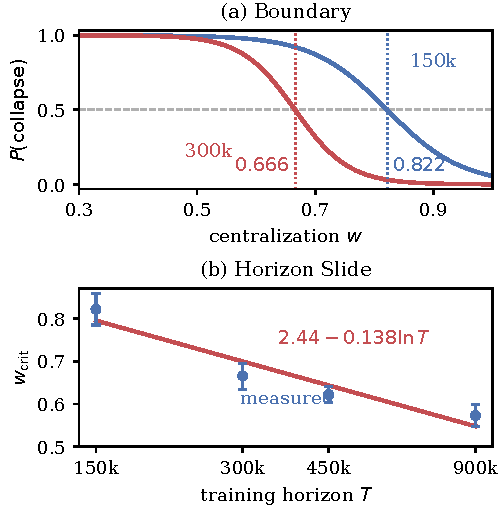
\includegraphics[width=\columnwidth]{Figures/boundary_metastability}
 \caption{Boundary location and horizon slide. (a)~At each fixed training budget, collapse probability
  changes steeply with reward centralization $w$; curves show fitted $P(\mathrm{collapse}\mid w)$ at two
  representative horizons (150k and 300k steps). (b)~All four measured horizons: increasing the
  training horizon shifts $\wcrit$ left, log-linearly in $T$ (RMSE $0.027$; 20 seeds per $w$-cell at
  each horizon), so more training rescues some runs that collapse at shorter horizons.}
 \label{fig:boundary}
\end{figure}

\begin{figure*}[t]
 \centering
 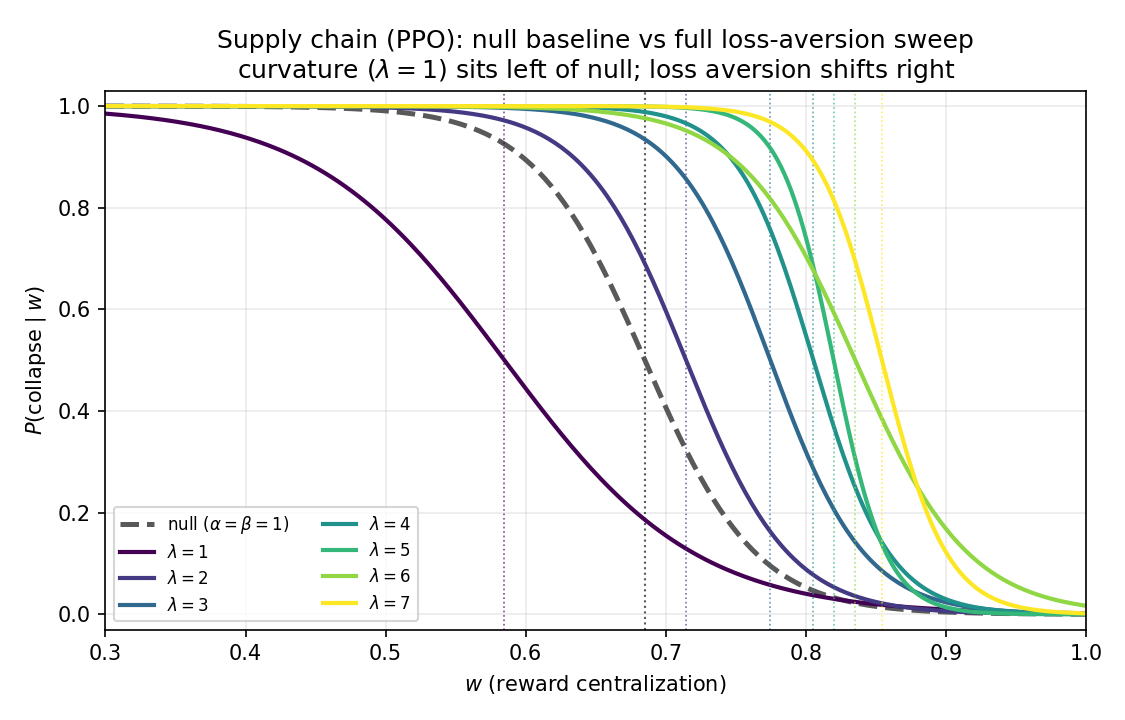
\includegraphics[width=0.6\textwidth]{Figures/ppo_behavioral_full}
 \caption{Loss aversion raises the collapse boundary (supply chain, PPO). Curves are fitted
  $P(\mathrm{collapse}\mid w)$; dotted lines mark $\wcrit$. Curvature alone
  ($\alpha{=}\beta{=}0.88$, $\lambda{=}1$) shifts the boundary \emph{left} of the linear
  baseline; increasing $\lambda$ then shifts it \emph{right}, saturating near
  $\wcrit\approx0.85$.}
 \label{fig:decomposition}
\end{figure*}

\begin{table}[t]
\centering
{\setlength{\tabcolsep}{3pt}\small
\begin{tabular}{lccccc}
\toprule
Condition & $\alpha,\beta$ & $\lambda$ & $\wcrit$ & vs.\ null & vs.\ curv. \\
\midrule
Linear null (rep.) & $1,1$ & 1 & 0.685 & -- & -- \\
Curvature & $0.88,0.88$ & 1 & 0.585 & $-0.100^{\checkmark}$ & -- \\
Loss av. & $0.88,0.88$ & 3 & 0.774 & $+0.089^{\checkmark}$ & $+0.189^{\checkmark}$ \\
Loss av. & $0.88,0.88$ & 7 & 0.854 & $+0.169^{\checkmark}$ & $+0.269^{\checkmark}$ \\
\bottomrule
\end{tabular}}
\caption{Decomposing reward-transform shifts (supply chain, PPO, 300k). ``vs.\ null'' is the
deployment shift against the reproduced linear baseline; ``vs.\ curv.'' is the isolated
loss-aversion shift against the curvature baseline. $\checkmark$ = difference CI excludes zero.}
\label{tab:decomposition}
\end{table}

The curvature result is scoped more narrowly: on the supply-chain PPO substrate, curvature and loss
aversion move $\wcrit$ in opposite directions (Table~\ref{tab:decomposition}); the transfer experiments
show the loss-aversion direction generalizes while the curvature sign does not. A speculative,
non-load-bearing account of \emph{why} the sign goes this way, an escape signal-to-noise argument, a
sign proposition resting on an unmeasured premise, an exploration-noise dissociation, and a
single-substrate summary curve, is given in full in the Supplement; none of it is required for, or
changes, the measurements above.

% =======================================================================
\section{The Instrument Travels; So Does the Direction}
\label{sec:generalization}

Beyond the supply chain, we estimate a CI'd $\wcrit$ in three further settings: the supply chain under
MAPPO (changing only the learner), and MPE and LBF under MAPPO (changing the environment). The design
is not fully crossed (parameter-shared PPO floors out on the shared-reward transfer tasks), so the
supply-chain/MAPPO cell is what separates the learner change from the environment change. In each we
ask whether the loss-aversion direction travels.

A transfer boundary is meaningful only if the learner can coordinate at high centralization.
Independent PPO fails this on the shared-reward transfer tasks: it collapses at \emph{every} $w$ on
both MPE and LBF (a coordination floor; Supplement), right-censoring the boundary rather than removing
it, whereas centralized-critic MAPPO~\citep{yu2022surprising} recovers coordination and exposes an
interior boundary. MPE has no native local--global conflict, so we construct one with a herding
wrapper (local reward for staying near others) and fix its scale, before the $\lambda$-sweep, so the
linear no-transform boundary is interior ($\wcrit=0.74$). MPE therefore tests whether the boundary
instrument and loss-aversion direction travel after changing the environment and learner; the absolute
thresholds remain conditional on this fixed wrapper and scale. Collapse is landmark occupancy below
$\theta=0.144$.

The loss-aversion direction transfers in every setting
(Figure~\ref{fig:generalization}, Table~\ref{tab:generalization}), reported at each setting's largest
interior $\lambda$ ($\lambda{=}7$ for supply and MPE, $\lambda{=}4$ for LBF, which saturates against
$w{=}1$ beyond that). On the \emph{supply chain under MAPPO} (only the
learner changes) $\wcrit$ rises $0.796\to0.889$, converging with PPO by $\lambda\!\geq\!4$; on
\emph{MPE} $0.78\to0.89$ ($+0.11$); on \emph{LBF} $0.26\to0.83$ by
$\lambda{=}4$. Secondary structure does
not transfer: on MPE the curvature shift spans zero ($+0.042$), and on LBF curvature moves the
boundary \emph{right} while the summary form misfits (RMSE $0.15$); so the portable claim is the CI'd
boundary and the loss-aversion direction, not the levels, curvature sign, or summary form.

\paragraph{Scope condition: action representation (single granularity tested).}
On the base-stock control the boundary depends on action granularity. Value-based learners (QMIX,
IQL) on a discretized $K{=}11$ shell give a flat collapse rate, but PPO on the \emph{same} shell also
goes flat (Table~\ref{tab:ablation}), so it is coarse discretization, not the value-based paradigm,
that erases the boundary; MPE, natively discrete yet retaining a boundary, shows this is coarseness
rather than discreteness per se. We tested only $K{=}11$, so we cannot yet distinguish the boundary
reappearing gradually as $K$ grows from it requiring near-continuous control specifically, which would
scope out value-based learners more fundamentally than ``coarse discretization'' suggests. A $K$-sweep
($K\in\{11,25,51,101\}$) would resolve this; untested here, so the loss-aversion \emph{direction} under
any value-based learner remains an open scope question, not a tested negative.

\begin{table}[t]
\centering
{\setlength{\tabcolsep}{5pt}\small
\begin{tabular}{lll}
\toprule
Learner & Action space & Boundary? \\
\midrule
PPO / MAPPO & continuous & yes \\
QMIX (centralized value) & discrete $K{=}11$ & no \\
IQL (independent value) & discrete $K{=}11$ & no \\
PPO (control) & discrete $K{=}11$ & \textbf{no} \\
\bottomrule
\end{tabular}}
\caption{Action-representation ablation. The last row is the key control: it changes only the action
space relative to continuous-control PPO, isolating coarse discretization as what erases the boundary.}
\label{tab:ablation}
\end{table}

\begin{figure*}[t]
 \centering
 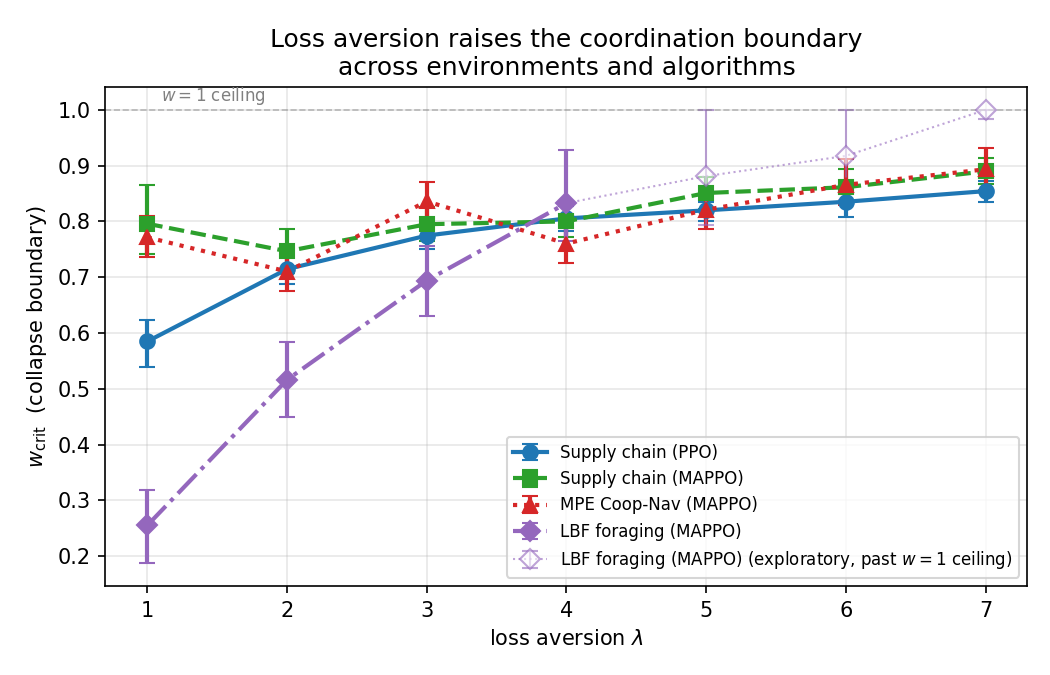
\includegraphics[width=0.7\textwidth]{Figures/generalization_wcrit_vs_lambda.png}%
 \caption{$\wcrit$ versus $\lambda$ across four settings: supply chain under PPO and MAPPO, MPE
  under MAPPO, LBF under MAPPO (bootstrap 95\% CIs). $\wcrit$ rises with $\lambda$ in every
  setting; the \emph{direction} generalizes, while levels (especially at $\lambda{=}1$), curvature
  sign, and exact form are substrate-specific. LBF $\lambda{\geq}5$ points extrapolate past the
  $w{=}1$ ceiling (outside the measured grid); they are drawn as hollow markers on a dotted
  line, visually distinct from the solid in-grid points, and are exploratory only.}
 \label{fig:generalization}
\end{figure*}

\begin{table}[t]
\centering
\small
\begin{tabular}{@{}lccc@{}}
\toprule
Setting & $\wcrit(\lambda{=}1)$ & $\wcrit$(last) & $\Delta$ \\
\midrule
Supply PPO   & \begin{tabular}[c]{@{}c@{}}$0.585$\\$[.545,.626]$\end{tabular} &
                \begin{tabular}[c]{@{}c@{}}$0.854$\\$[.837,.871]$\end{tabular} & $+0.269$ \\
Supply MAPPO & \begin{tabular}[c]{@{}c@{}}$0.796$\\$[.742,.860]$\end{tabular} &
                \begin{tabular}[c]{@{}c@{}}$0.889$\\$[.856,.917]$\end{tabular} & $+0.093$ \\
MPE MAPPO    & \begin{tabular}[c]{@{}c@{}}$0.78$\\$[.73,.83]$\end{tabular} &
                \begin{tabular}[c]{@{}c@{}}$0.89$\\$[.84,.93]$\end{tabular} & $+0.11$ \\
LBF MAPPO    & \begin{tabular}[c]{@{}c@{}}$0.26$\\$[.20,.32]$\end{tabular} &
                \begin{tabular}[c]{@{}c@{}}$0.83$\\$[.78,.89]$\end{tabular} & $+0.57$ \\
\bottomrule
\end{tabular}
\caption{Generalization of the loss-aversion \emph{direction}. Within-sweep endpoints
($\alpha{=}\beta{=}0.88$) with bootstrap 95\% CIs, $\lambda{=}1\to$last interior (LBF: $\lambda{=}4$);
$\Delta$ is the endpoint difference.}
\label{tab:generalization}
\end{table}

% =======================================================================
\section{A Single Downstream Node Can Nearly Set the Boundary}
\label{sec:minority}

This experiment is necessarily supply-chain-only: it requires a directed resource-flow topology (a
DAG) that MPE and LBF lack. The main sweep is homogeneous; here we make one node loss-averse while
the others stay risk-neutral, holding everything else identical to the main sweep, and ask whether
one biased node can move the boundary and whether its position sets the shift. Position could matter
because the network is a branching DAG: demand
enters at the retail edge, two downstream nodes feed it directly, and upstream suppliers feed one or
both paths, so a node should matter more when its output reaches demand through a short, concentrated
path. Because MPE and LBF lack this topology, the heterogeneous-node effect is tested here only on
the supply chain.

\paragraph{A single node, dose for dose.}
Sweeping the most downstream node's $\lambda\in\{1,\dots,7\}$ (others risk-neutral) traces a strictly
monotone dose-response: $\wcrit$ rises $0.585\to0.863\,[0.846,0.880]$, matching the \emph{fully}
loss-averse (homogeneous) value ($0.854\,[0.837,0.871]$) within noise (CIs overlap) by $\lambda{=}7$
with the same saturating shape as the homogeneous sweep. Operationally, the
team's collapse boundary is not an average over agents: a single node's reward design can nearly set it
on its own, so an audit of reward transforms should not treat the boundary as an average over agents.
Which node matters most is position-dependent under a shared actor but does not survive as a general
rule once the shared gradient is removed (below).

\paragraph{Position: proximity to demand, not chain index, under a shared actor.}
Placing one $\lambda{=}7$ node at each position, the effect is strongly position-dependent, and under
the shared-parameter actor the observed ordering is consistent with how directly a node's output
reaches demand, not a chain index. The two
retail-feeding nodes dominate ($0.863$, $0.800$); the sole supplier to the dominant downstream node is
comparable within noise ($0.797$); the split-path suppliers are weaker ($0.726$, $0.673$, also
overlapping each other). Because a single shared actor can let a biased node's gradient influence
others' behavior directly, and because nodes at different positions encounter different observations,
visitation, and advantage distributions even under a common observation format, this ordering is not
by itself evidence that the mechanism is topological: we designed a second, independently-parameterized
sweep specifically to test this before drawing that conclusion.

\paragraph{The ordering does not survive without a shared gradient.}
We repeat the identical position sweep with five fully independent PPO actors, one per trainable node,
each updated only on its own transitions and sharing no parameters or gradient with the others (same
env, $w$-grid, seeds, $\alpha,\beta,\lambda$, label, and estimator; each actor trains for $60$k real
environment ticks, matching the shared actor's per-agent exposure). This is not a reshuffling: the
previously dominant node ($0.863$, rank 1)
becomes the weakest of the five ($0.498\,[0.363,0.581]$, rank 5), while the previously weakest node
(rank 5) rises to rank 2 (Table~\ref{tab:cascade_compare}). The coarse retail-adjacent-vs-split-path
grouping also fails to replicate (mean $0.832$ vs.\ $0.700$ under the shared actor; $0.606$ vs.\ $0.553$,
no longer cleanly separated, under separate actors). We conclude the position-specific ordering under
the shared actor is substantially a shared-gradient artifact rather than evidence for a directed
product-flow mechanism, and we do not draw a topological reading from it. Where \citet{mengesha2025}
find loss aversion's effect on cooperation is \emph{non-monotone} in an evolutionary model, the sign of
the effect here (loss aversion raises $\wcrit$) is monotone and, unlike the position ordering, is not
an artifact of parameter sharing (Table~\ref{tab:decomposition}).

\begin{table}[t]
\centering\small
\begin{tabular}{@{}lcccc@{}}
\toprule
Position & Shared & Rank & Separate & Rank \\
\midrule
node\_2 & \begin{tabular}[c]{@{}c@{}}$0.863$\\$[.846,.880]$\end{tabular} & 1 &
          \begin{tabular}[c]{@{}c@{}}$0.498$\\$[.363,.581]$\end{tabular} & 5 \\
node\_3 & \begin{tabular}[c]{@{}c@{}}$0.800$\\$[.780,.820]$\end{tabular} & 2 &
          \begin{tabular}[c]{@{}c@{}}$0.714$\\$[.683,.745]$\end{tabular} & 1 \\
node\_5 & \begin{tabular}[c]{@{}c@{}}$0.797$\\$[.740,.857]$\end{tabular} & 3 &
          \begin{tabular}[c]{@{}c@{}}$0.538$\\$[.474,.591]$\end{tabular} & 4 \\
node\_6 & \begin{tabular}[c]{@{}c@{}}$0.726$\\$[.682,.769]$\end{tabular} & 4 &
          \begin{tabular}[c]{@{}c@{}}$0.547$\\$[.495,.594]$\end{tabular} & 3 \\
node\_4 & \begin{tabular}[c]{@{}c@{}}$0.673$\\$[.622,.720]$\end{tabular} & 5 &
          \begin{tabular}[c]{@{}c@{}}$0.559$\\$[.502,.608]$\end{tabular} & 2 \\
\bottomrule
\end{tabular}
\caption{Position sweep, shared vs.\ separate actors ($\lambda{=}7$, $n{=}20$/position/actor
condition). Rank 1 = strongest effect on $\wcrit$. Shared and separate columns report $\wcrit$ with
bootstrap 95\% CIs.}
\label{tab:cascade_compare}
\end{table}

% =======================================================================
\section{Discussion}
\label{sec:discussion}

To our knowledge no prior work separates the transform's curvature and loss-aversion components in
cooperative MARL~\citep{lalmohammed2025,ghaemi2024risk}. On the supply-chain PPO substrate the two move
the boundary in \emph{opposite} directions and would partially cancel if reported jointly, so a single
``prospect-theoretic'' condition under-reports the loss-aversion effect by about half there; the
curvature sign itself is supply-chain-specific and not measured to transfer: it spans zero on MPE and
runs the \emph{same} direction as loss aversion on LBF.

The boundary is a design quantity: a team can budget for the loss-aversion margin rather than discover
collapse in production: if $w$ is capped at, say, $0.8$, the usable budget is where $\wcrit$ crosses
that cap, about $\lambda\approx4$ here. The minority result shows a single node's reward design can
nearly set the whole team's boundary, so an audit of reward transforms should not treat the boundary as
an average over agents; identifying \emph{which} node matters most is system-specific (the deconfounded
sweep above rules out a general position rule) and whose dual-use we address in the ethics statement.

\paragraph{Scope and Future Work.}
Three limits point to next steps. The quantitative core is single-substrate (magnitudes belong to one
simulator, the summary form does not transfer), and the minority-node sensitivity is not cleanly a
directed-flow effect (the deconfounded sweep rules out a general position rule on this substrate), so
the open question is narrower than a second directed-flow domain: whether minority-agent boundary
dominance under parameter sharing transfers across networks and learning architectures, not whether a
positional cascade does. The mechanism fixes sign but not magnitude: localizing $\wcrit$ from
dynamics resisted two pre-committed probes, so a localizing observable is the clearest
open problem. And $\varrho$ only partially compensates for reward-unit dependence; finding a fully
unit-invariant coordinate, or showing none exists for this class of transforms, is as open a problem
as localizing $\wcrit$ itself.

% =======================================================================
\section{Conclusion}
\label{sec:conclusion}

Reward centralization is usually treated as a direction: more team signal helps. We have shown it also
has a measurable location, a critical mixture $\wcrit$, that moves rightward under loss-averse
transforms and leftward with longer training, and that a single node's reward design can nearly set it
on its own under parameter sharing, a sensitivity that a deconfounded, independently-parameterized
sweep shows is not a general topological rule. The direction and horizon slide generalize; the
thresholds are system-specific, but the protocol is not.

% =======================================================================
\section*{Ethical Statement}

This work is entirely simulated, with no human subjects or personal data. Reported thresholds are
substrate-specific and must be re-measured before use; the minority-node result is dual-use
(hardening vs.\ targeted disruption), reported explicitly for auditability.

% =======================================================================
\bibliography{references}

\end{document}
